\documentclass[letterpaper,12pt]{article}
\usepackage[margin=1in]{geometry}
\usepackage{libertine}
\usepackage{parskip}
\usepackage{graphicx}
\pagestyle{empty}
\begin{document}

\hspace*{-1in}

\includegraphics[scale=0.9]{CoverPage.jpg}

\title{Two Graph Vertex Partitioning Algorithms for Part Consolidation in Axiomatic Design}
\author{Jeffery Cavallaro}
\date{13 August 2019}
\maketitle
\section*{Abstract}
In traditional manufacturing, parts are designed and manufactured separately so that the parts can be combined into
subassemblies, which are then combined into final assemblies.  Indeed, the standardization of parts was one of the key
developments that fueled the explosive growth of manufacturing during the \(19^{th}\) and \(20^{th}\) centuries.  Now, in the
\(21^{st}\) century, a new technique, referred to as \emph{additive manufacturing}, promises a new leap in manufacturing
capability: instead of manufacturing the parts for subassemblies separately, the subassemblies are constructed directly
through the additive application of layers of material, commonly referred to as \emph{3-D printing}.

But what is the best way to allocate parts into subassemblies in order to minimize the number of subassemblies?  One possible
answer is to represent the problem by a graph, where the nodes are the parts and the edges represent the need to separate
incident parts into different subassemblies.  The answer then becomes the solution to a standard proper coloring problem.  So
what is needed is a rationale for determining the presence of an edge.  A good way to determine the separation of two parts
into different subassemblies is through the use of so-called \emph{axiomatic design}, where a set of \emph{design parameters}
(DPs) are translated into a set of \emph{functional requirements} (FRs) via a \emph{design matrix} (A) of common and
problem-specific axioms: \([FR]=[A][DP]\).

The primary goal of this research project is to study and improve upon existing algorithms related to the \(k\)-coloring of
graphs related to additive manufacturing that are obtained using the principles of axiomatic design.  Since previous work has
relied on manual execution of the algorithms under study, an additional goal is to develop software solutions that can extend
the ability to try and compare various examples.

\section*{Timeline}

Note: Some tasks to run concurrently.

\begin{tabular}{|l|c|}
  \hline
  \textbf{Topic} & \textbf{weeks} \\
  \hline
  Reading on Axiomatic Design & 3 \\
  Reading on Additive Manufacturing & 2 \\
  Reading on k-Colorable Determination Algorithms & 2 \\
  Reading on Proper Coloring Algorithms & 1 \\
  Existing Algorithm Analysis & 2 \\
  Algorithm Improvement & 4 \\
  Algorithm Software Development & 2 \\
  Published Paper Support & 4 \\
  \hline
\end{tabular}

\section*{Reading List}

\begingroup
\renewcommand{\section}[2]{}%
\nocite{*}
\bibliographystyle{amsplain} 
\bibliography{ref}
\endgroup

\hspace*{-1in}
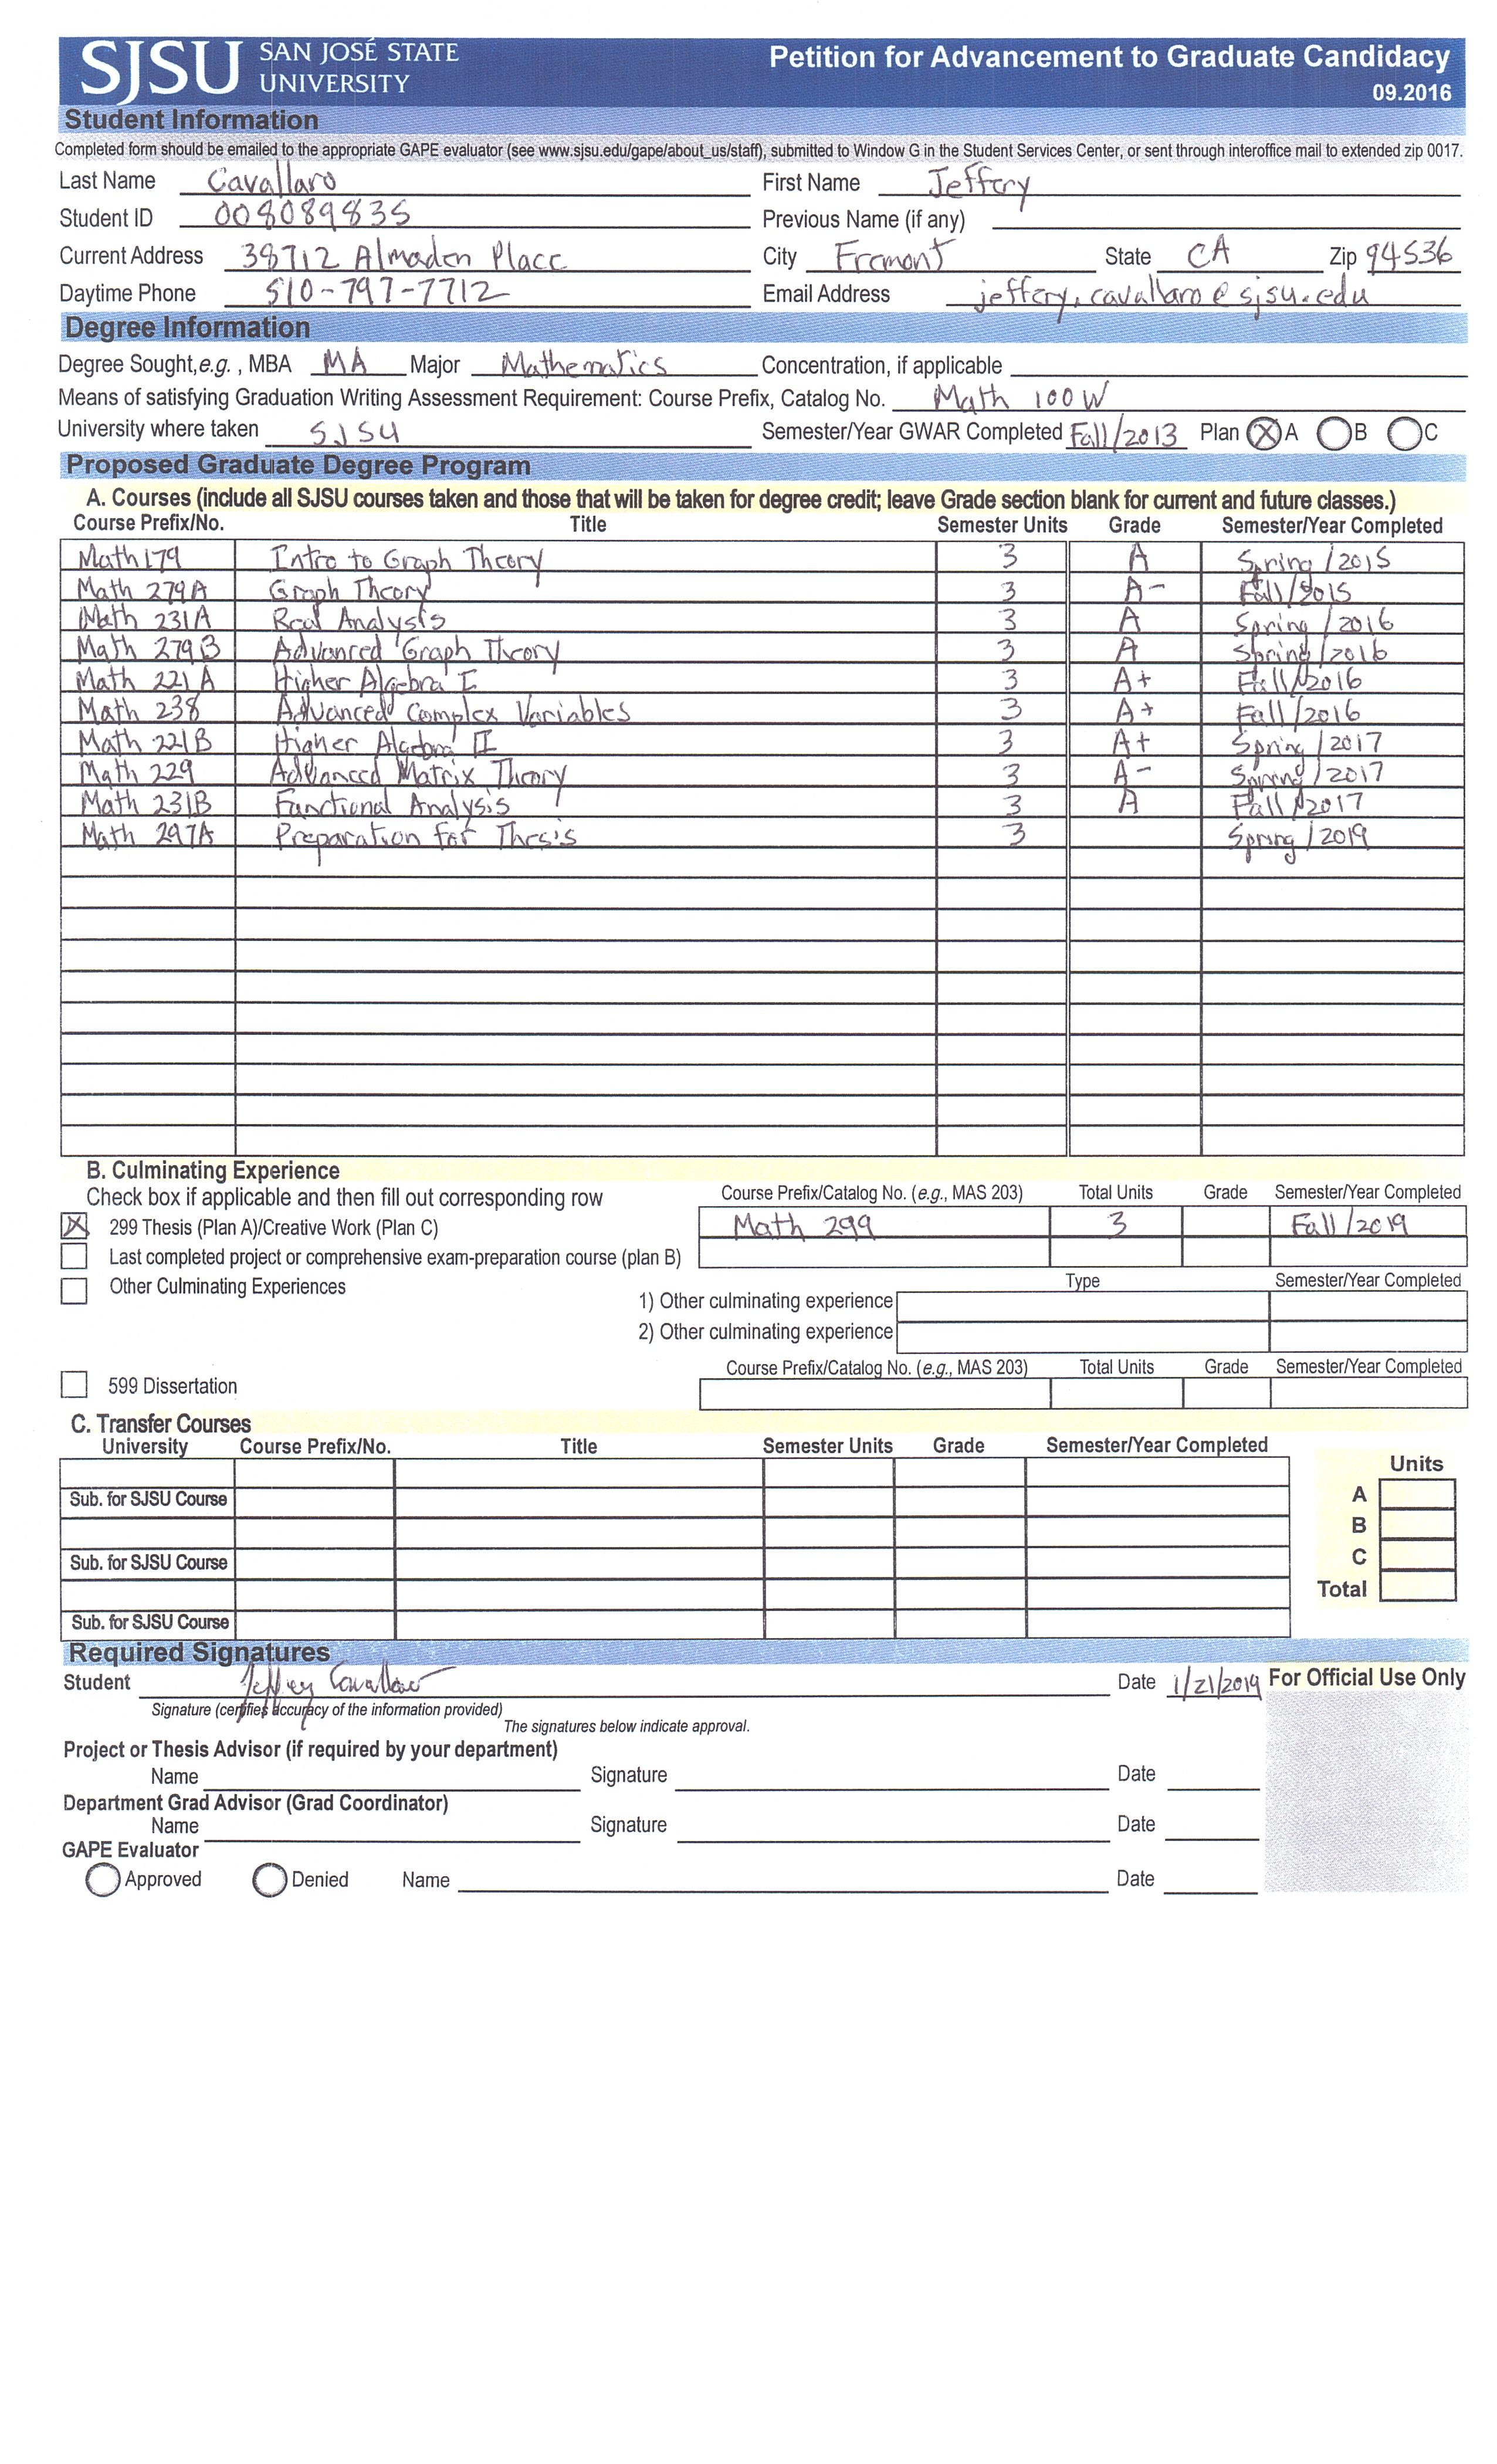
\includegraphics[scale=0.9]{candidacy.jpg}

\end{document}
